\chapter{Estado del arte}
\label{chapter:estado_del_arte}


\section{Recomendadores actuales}

\paragraph{}
A día de hoy, existen multitud de clasificadores y recomendadores\cite{ref:sorter_art_1} que se usan a diario para realizar todo tipo de recomendaciones, que van desde cual es el mejor producto en base a unas necesidades, pasando por clasificar piezas o productos en una fabrica para organizar la disponibilidad de estas, hasta incluso a recomendadores de canciones, series o películas en base a unas características de quien solicita estas.

\paragraph{}
Esto se ha conseguido gracias a la investigación y al IOT (Internet de las cosas 'Internet of Things') que facilita la vida a los investigadores y sobre todo a las personas. Antiguamente eran los usuarios los que, si querían comparar algo, tenían que buscar y buscar por tiendas para encontrar, o bien el mismo producto a distintos precios o bien productos alternativos al que quería adquirir o que directamente desconocía de la existencia de esa alternativa. Esto le consumía muchas horas (o incluso días) y ademas no tenia la garantía de haber abarcado todas las posibilidades\cite{ref:traditional_purchase_internet_purchase}.

\paragraph{}
Hoy en día, a través de Internet y gracias a los Recomendadores/Clasificadores actuales, el usuario puede consultar todas las alternativas y precios y estar mas seguro de que hace una buena elección antes de hacer la inversión\cite{ref:internet_comparatives}.

\paragraph{}
Los sistemas de recomendación/clasificación existen desde hace muchos años\cite{ref:history_recommender}. Han estado ahí para ayudarnos sin darnos cuenta, aunque al principio fueron muy rudimentarios. A medida que las características y el volumen de opciones crecía, se hacia mas complicado y lento realizar esa clasificación/recomendación. Y en ese punto es donde entro los algoritmos de aprendizaje automático (\textit{Machine Learning}) para ayudar a que esas clasificaciones y recomendaciones fueran posibles en un tiempo razonable.

\paragraph{}
Dos empresas que quizás merezcan mención especial (gracias a la fama que consiguieron al implementar estos algoritmos) son \textit{Spotify}\cite{ref:music_recommender} con su recomendador de canciones y \textit{Netflix}\cite{ref:netflix} con su recomendador de series. Ambos utilizan el poder de los algoritmos de recomendadores de \textit{Machine Learning} para analizar el comportamiento que tienen sus usuarios en las correspondientes plataformas y sugerir recomendaciones basándose en estos comportamientos.


\subsection{Recomendadores en el ámbito de la medicina}
Pese a que en el ámbito de la medicina se ha utilizado mucho la estadística, el uso de estos recomendadores ha sido mas discreto, o al menos no se ha dado a conocer su uso al publico potencial, llegando a quedarse en la fase de caso de estudio sin llegar a convertirse en un producto final. Un ejemplo de esto es el recomendador de medicamentos personalizado\cite{ref:refer_medical_prescriptions} que se basa en el historial clínico del paciente para recomendar la medicación que se ha de tomar este. Este es un caso de uso muy similar a nuestro \hyperref[op:OP1]{OP1}, aunque en nuestro caso, buscamos recomendar referencias bibliográficas clínicas.

\paragraph{}
También se conocen casos donde se han usado estos Clasificadores/Recomendadores para clasificar muestras o grupos de individuos para realizar un posterior análisis del grupo, como por ejemplo este caso de uso\cite{ref:refer_classify_plaquetas} que utiliza un clasificador para clasificar plaquetas para un posterior ensayo medico.

\paragraph{}
Todo y con eso, como comentamos anteriormente, el uso de Clasificadores/Recomendadores en este ámbito suele pasar a estar en segundo plano por lo que se ha de intuir su uso para darse cuenta que sin ellos, muchos estudios no serian posibles a día de hoy.

\newpage
\subsection{Recomendadores en el ámbito de la salud}

\paragraph{}
Al igual que en el caso anterior, el uso de recomendadores en el ámbito de la salud pasa desapercibido y es raro la vez que se destaque como solución final para la ayuda a los profesionales sanitarios.

\paragraph{}
A continuación destacamos los más conocidos en este ámbito:

\paragraph{• Pubmed\cite{ref:pubmed_home}:}  Esta web Creada por el Centro Nacional de Biotecnología \textit{National Center for Biotechnology Information (NCBI)} Permite hacer búsquedas por texto libre y permite realizar filtros por año, tipo de artículo y disponibilidad del texto. En el listado también se puede observar el estado de los artículos, si la publicación es definitiva o aun se esta revisando su contenido. El orden de los resultados es por aproximación al texto que se busque (mejor acierto), aunque permite modificar la ordenación por fecha del artículo, nombre de autor u origen del artículo. En las figuras \ref{fig:pubmed1} y \ref{fig:pubmed2} puede ver el aspecto de la pagina y los resultados de una búsqueda.

\begin{figure}[h!]
    \begin{subfigure}[b]{0.45\linewidth}
    	\centering
		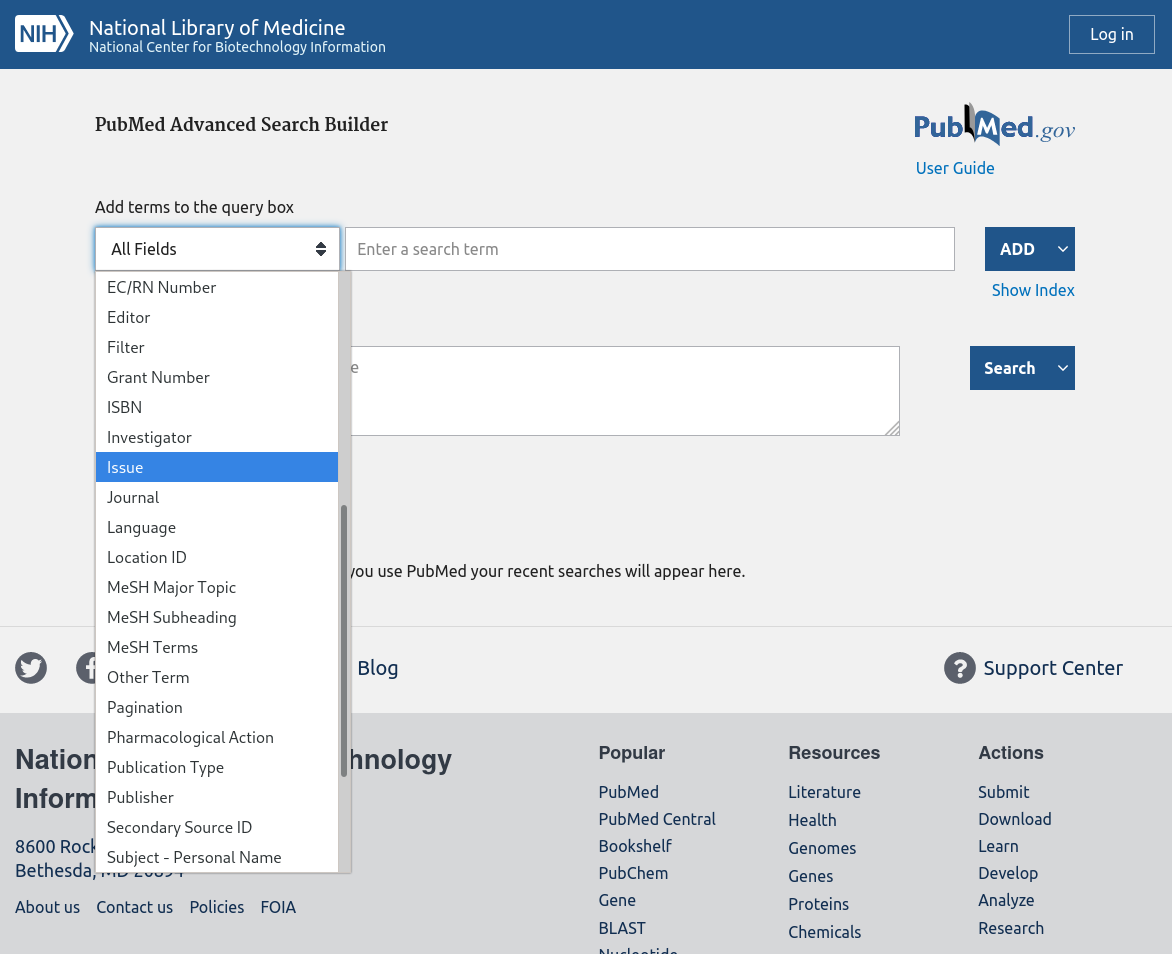
\includegraphics[width=0.9\textwidth]{images/Pubmed.png}
		\caption{Vista principal de Pubmed.}
		\label{fig:pubmed1}
	\end{subfigure}
	\begin{subfigure}[b]{0.45\linewidth} 
		\centering
		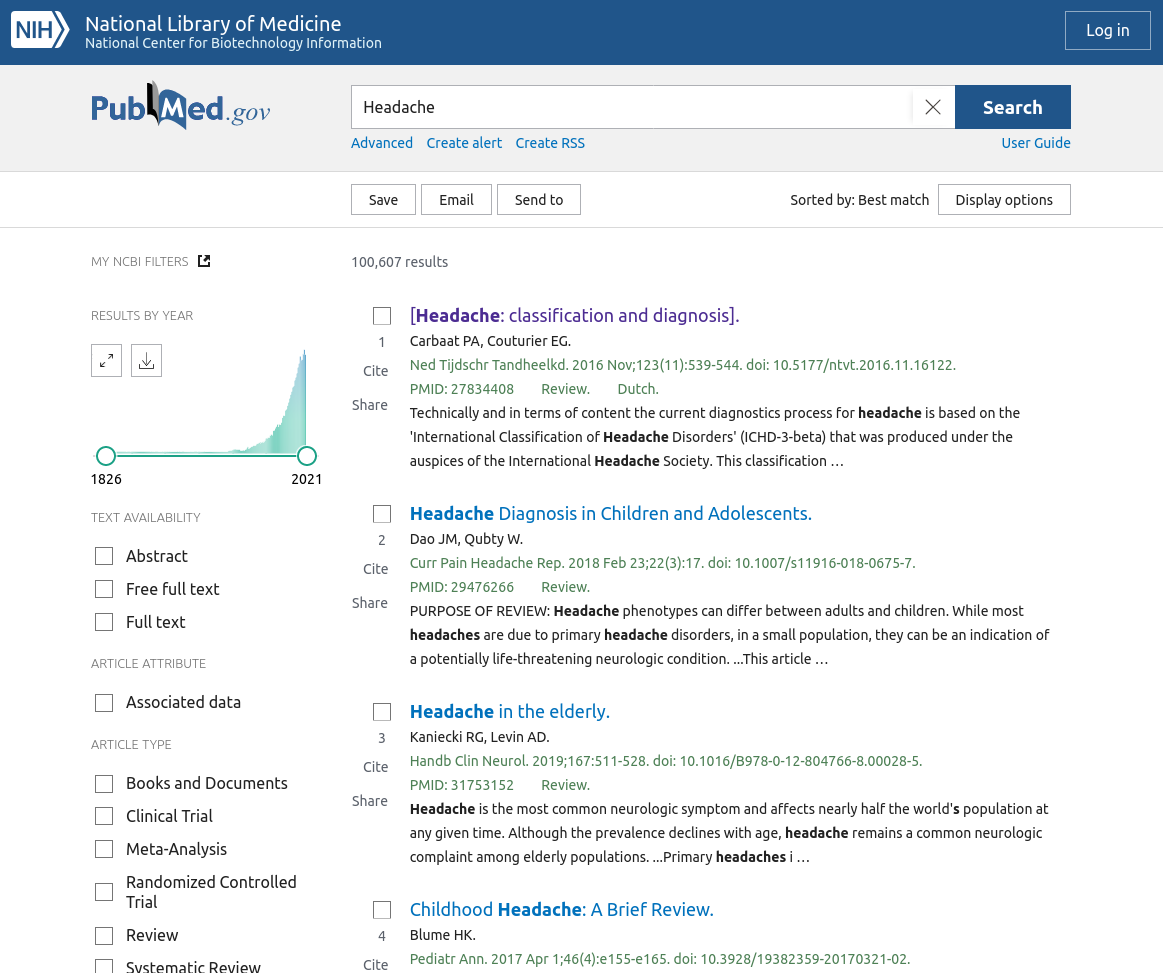
\includegraphics[width=0.9\textwidth]{images/Pubmed2.png}
		\caption{Resultados de búsqueda de Pubmed.}
		\label{fig:pubmed2}
	\end{subfigure}
	\caption{Web de Pubmed.}
	\label{fig:pubmed}
\end{figure}

\newpage
\paragraph{• ClinicalTrials\cite{ref:clinicaltrials_home}:} Esta web es una base de datos de estudios clínicos financiados con fondos públicos y privados realizados en todo el mundo. Permite realizar búsquedas y filtrados complejos de dolencias, mostrando los resultados en formato lista ordenados por fecha mas reciente, aunque el usuario puede elegir otras ordenaciones y filtrados. El listado también muestra el estado del documento (si ya esta finalizada la investigación o aun esta en proceso) y otra información relevante como el tratamiento que se esta aplicando. En las figuras \ref{fig:clinical_trials1} y \ref{fig:clinical_trials2} puede ver el aspecto de la pagina y los resultados de una búsqueda.

\begin{figure}[h!]
   	\centering
	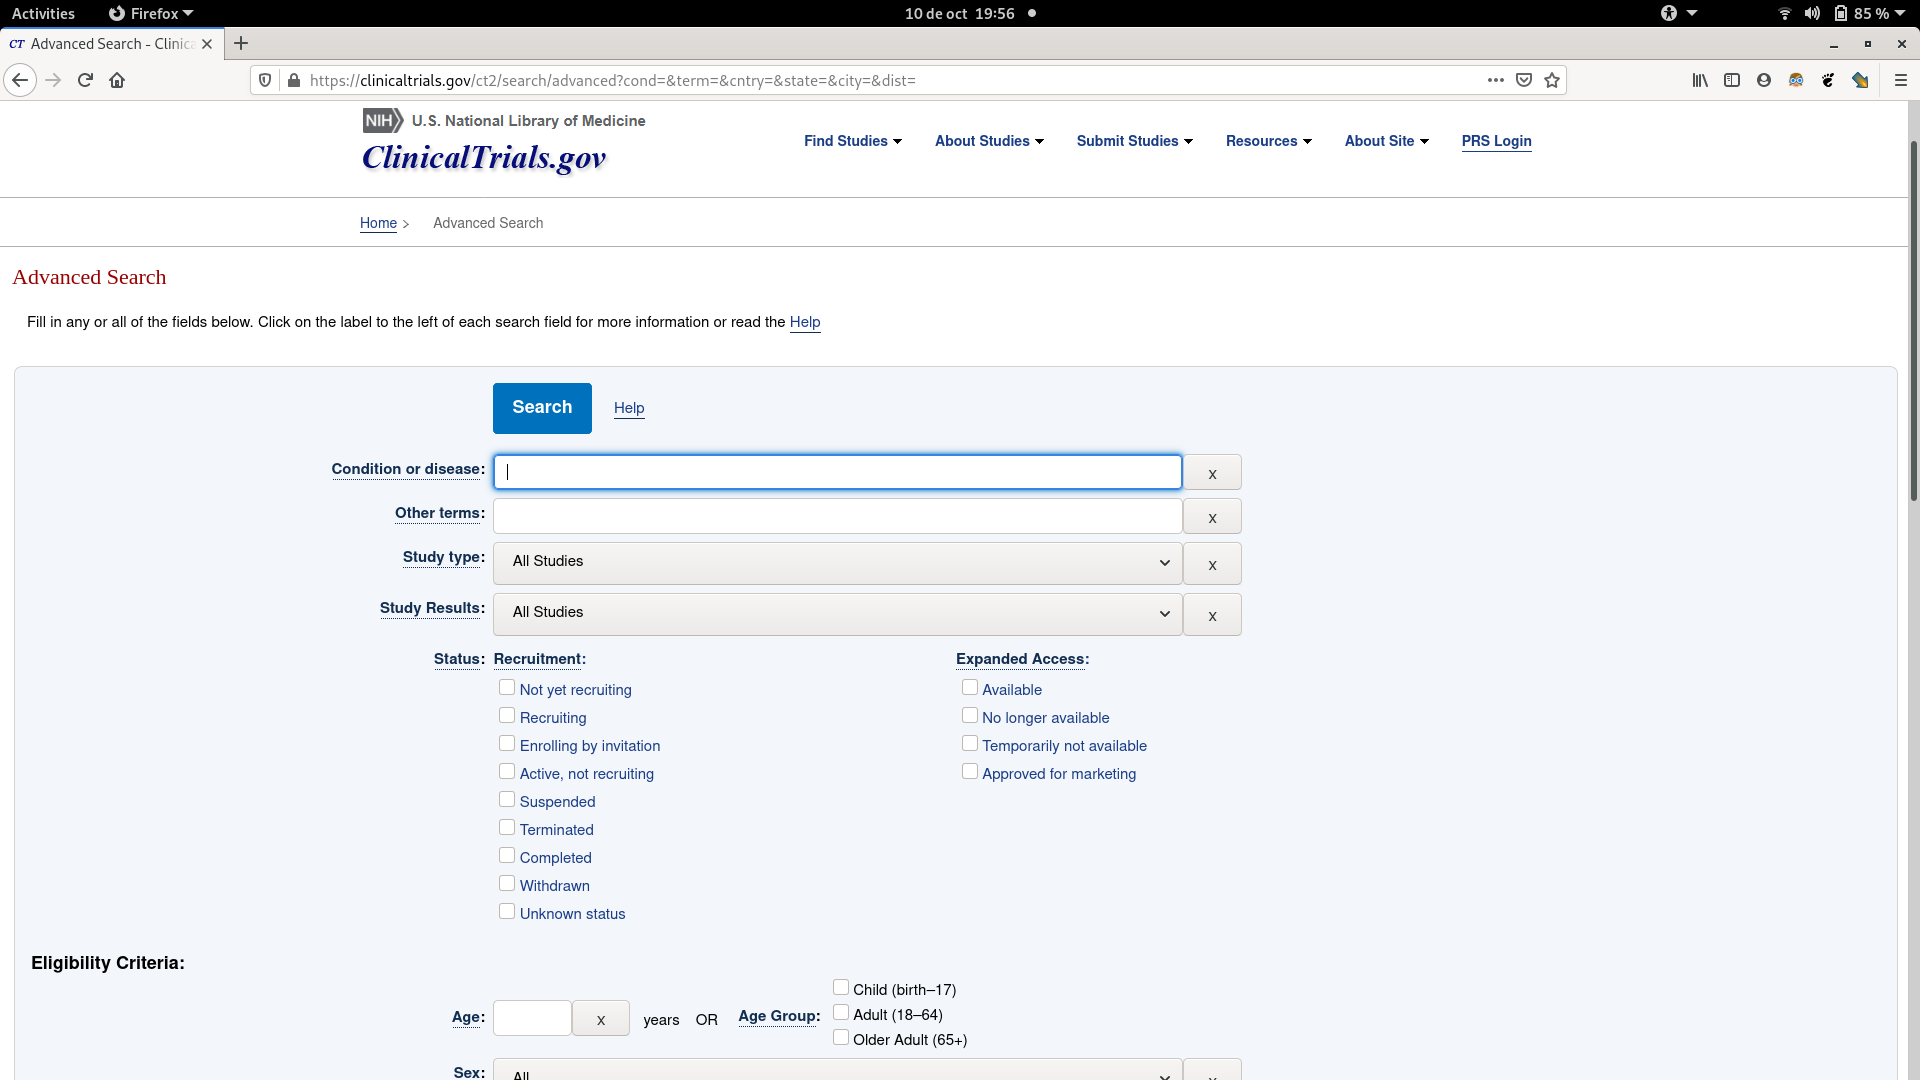
\includegraphics[width=0.7\textwidth]{images/ClinicalTrials.png}
	\caption{Vista principal de ClinicalTrials.}
	\label{fig:clinical_trials1}
\end{figure}

\begin{figure}[h!]
	\centering
	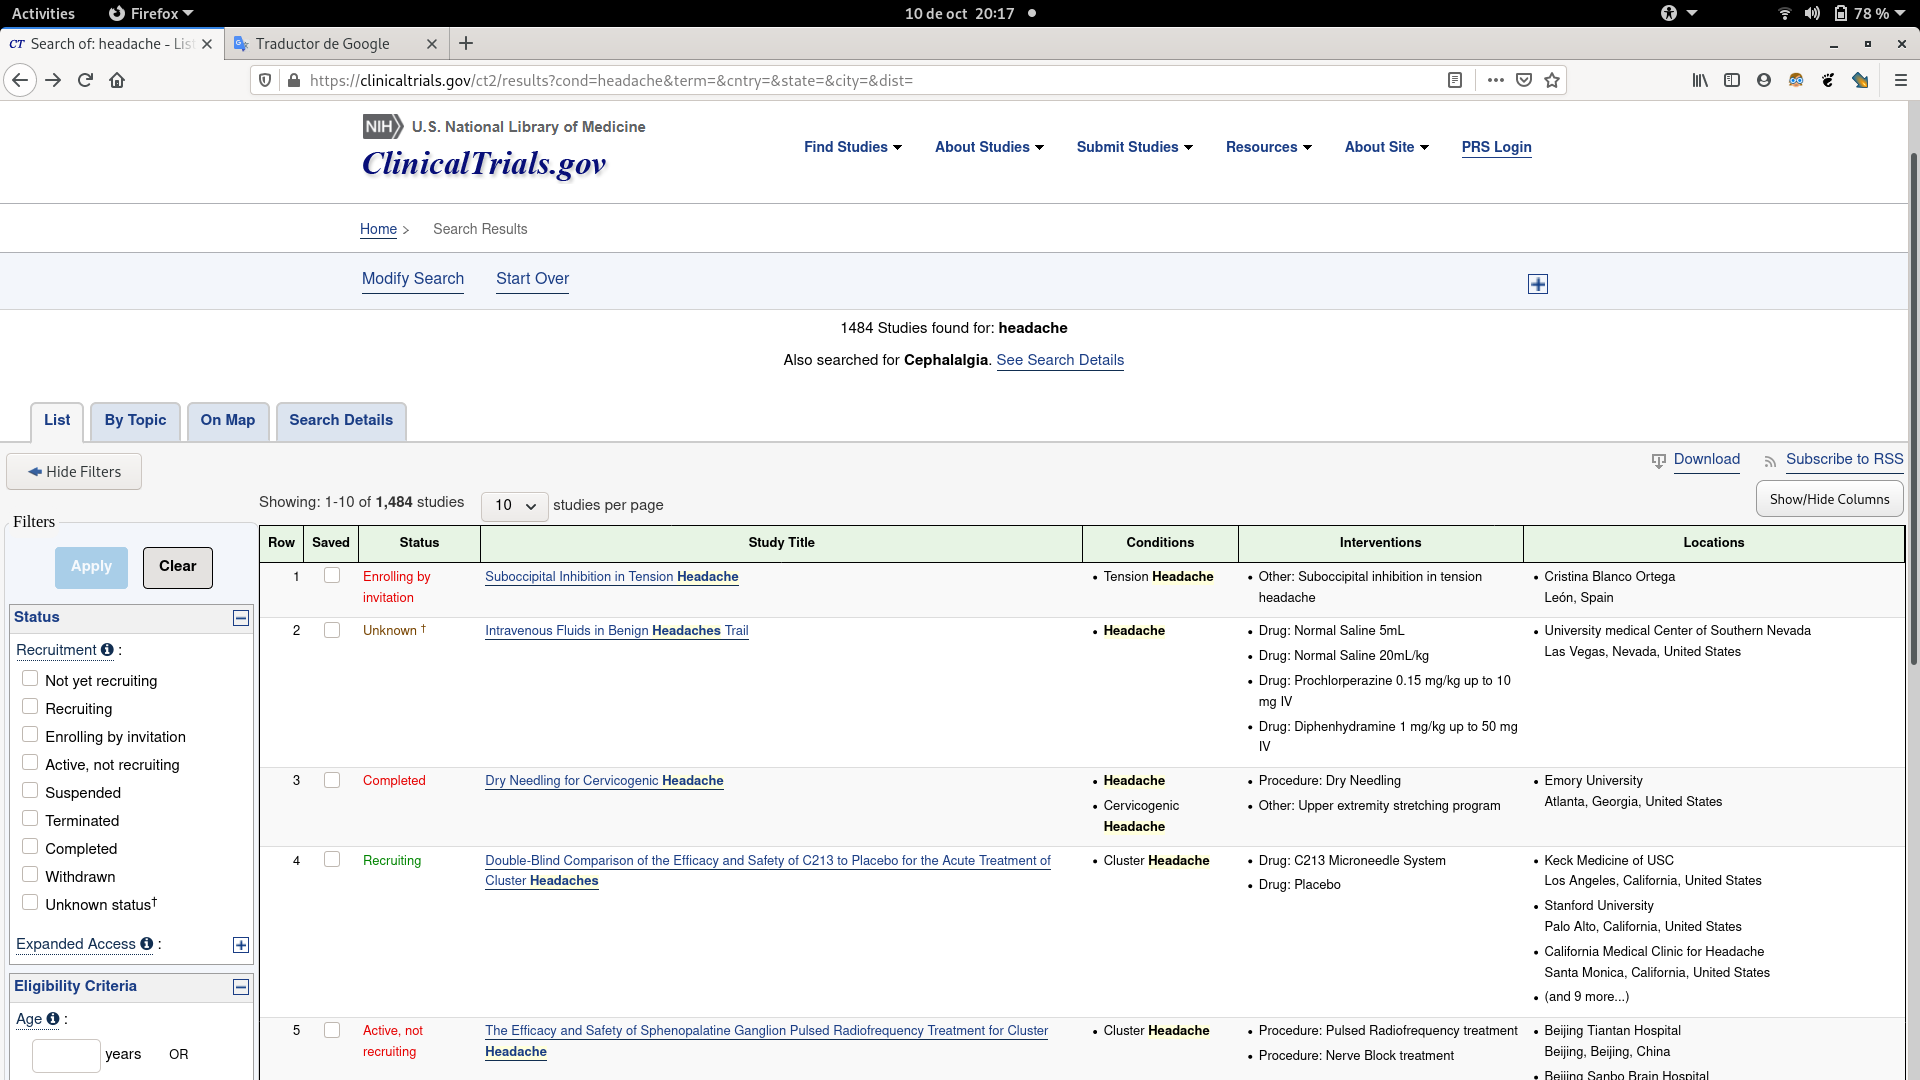
\includegraphics[width=0.7\textwidth]{images/ClinicalTrials2.png}
	\caption{Resultados de búsqueda de ClinicalTrials.}
	\label{fig:clinical_trials2}
\end{figure}

\newpage
\paragraph{• MedlinePlus\cite{ref:medlineplus_home}:} Esta web creada por Biblioteca Nacional de Medicina de EE. UU. (NLM, por sus siglas en inglés), esta más orientada al paciente que las anteriores, y permite buscar artículos médicos basándose en texto relacionado. Por ejemplo si ponemos un tipo de síntoma en el buscador, este nos muestra artículos relacionados con ese texto como si de un buscador de Internet común se tratara, aunque a diferencia de estos, MedlinePlus promete brindar información de calidad y relevante de salud y bienestar que sea confiable y fácil de entender. Aparentemente este buscador muestra los resultados en orden de relevancia aunque, igual que en los casos anteriores, no permite valorar si esos artículos son realmente interesantes para la búsqueda relacionada.En las figuras \ref{fig:medlineplus1} y \ref{fig:medlineplus2} puede ver el aspecto de la pagina y los resultados de una búsqueda.

\begin{figure}[h!]
    \begin{subfigure}[b]{0.45\linewidth}
    	\centering
		
\includegraphics[width=0.9\textwidth]{images/MedlinePlus.png}
		\caption{Vista principal de MedlinePlus.}
		\label{fig:medlineplus1}
	\end{subfigure}
	\begin{subfigure}[b]{0.45\linewidth} 
		\centering
		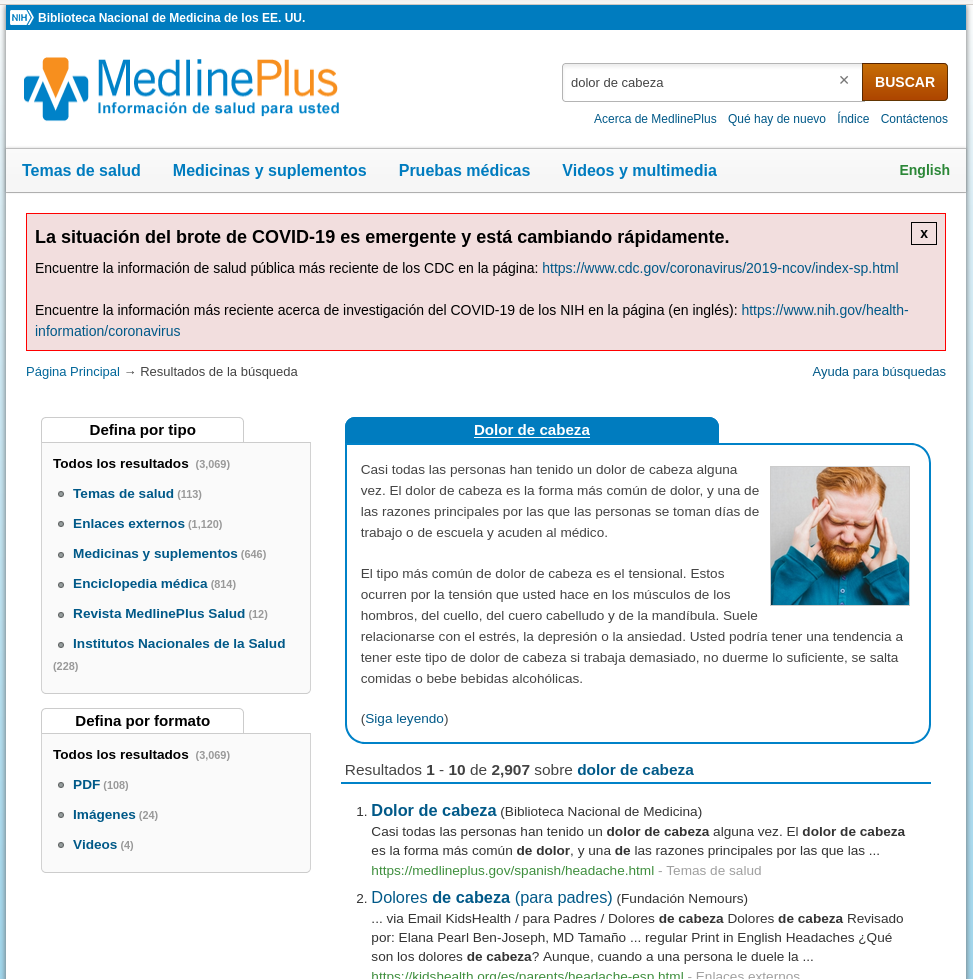
\includegraphics[width=0.9\textwidth]{images/MedlinePlus2.png}
		\caption{Resultados de búsqueda de MedlinePlus.}
		\label{fig:medlineplus2}
	\end{subfigure}
	\caption{Web de MedlinePlus.}
	\label{fig:medlineplus}
\end{figure}

\newpage
\section{Recomendadores en el futuro}

\paragraph{}
Los recomendadores/clasificadores han ayudado mucho en la medicina, sobre todo en el ámbito de la investigación, en donde se requiere un trabajo previo para poder tener un conjunto de datos valido para el posterior estudio que se quiera realizar. En el caso que nos toca, ayudara a los profesionales sanitarios a poder encontrar otras referencias bibliográficas clínicas de otros casos similares al que tienen, para así poder valorar alternativas, cosa que sin estos recomendadores/clasificadores, seria un trabajo eterno de realizar, por no decir casi imposible, debido al gran volumen de información que cada día se genera. Estos algoritmos de recomendación/clasificación, no solo seguirán siendo un pilar básico en el ámbito medico, sino que seguramente aparecerán nuevos algoritmos de clasificación/recomendación que facilitaran las futuras investigaciones, como ya se esta observando en los nuevos recomendadores para el control de la glucosa en la sangre\cite{ref:refer_diabetes_control}.
